\section{Testing}
Dopo aver visto come configurare i partecipanti alla VPN, si passa a descrivere
i test che ho effettuato per verificare che il tutto funzionasse.

\subsection{Test 1}
Il primo test è stato eseguito sulla configurazione spiegata all'inizio del capitolo,
eccola spiegata nel dettaglio:
\begin{itemize}
  \item OpenVPN server ospitato su AWS, raggiungibile da nome DNS, sistema
  operativo \texttt{Ubuntu Server}, indirizzo IP privato \texttt{172.31.40.221}
  \item \textit{Docker host} ospitato su AWS, nella stessa rete privata del
  server, sistema
  operativo \texttt{Ubuntu Server}, indirizzo IP privato \texttt{172.31.43.141}
  \item due reti virtuali, create con VirtualBox:
  \begin{itemize}
    \item rete 1, detta \texttt{net50}, costituita da:
    \begin{itemize}
      \item firewall stateful, NAT verso l'esterno e traffico consentito solo
      sulle porte 80 e 443 TCP, indirizzo IP \texttt{192.168.100.254},
      sistema operativo \texttt{Alpine Linux}
      \item client VPN, sistema operativo \texttt{Ubuntu desktop}, indirizzo
      IP \texttt{192.168.100.20}, default gateway \texttt{192.168.100.254}
      \item due host \texttt{Alpine Linux}, indirizzi IP rispettivamente
      \texttt{192.168.100.30} e \texttt{192.168.100.40}, entrambi con un server
      web in ascolto sulla porta 80
    \end{itemize}
    \item rete 2, detta \texttt{net200}, costituita da:
    \begin{itemize}
      \item firewall stateful, NAT verso l'esterno e traffico consentito solo
      sulle porte 80 e 443 TCP (e 53 UDP -- DNS), indirizzo IP
      \texttt{192.168.100.254},
      sistema operativo \texttt{Alpine Linux}
      \item client VPN, sistema operativo \texttt{Ubuntu desktop}, indirizzo
      IP \texttt{192.168.100.20}, default gateway \texttt{192.168.100.254}
      \item un host \texttt{Alpine Linux}, con indirizzo IP
      \texttt{192.168.100.30} ed un server
      web in ascolto sulla porta 80\footnote{Non ho usato un secondo host anche
      in questa rete perché il carico di lavoro del mio portatile iniziava ad
      essere un pò elevato.}
    \end{itemize}
  \end{itemize}
\end{itemize}
Le due reti sono state appositamente scelte uguali per testare il funzionamento
dell'\textit{IP mapping}. In particolare:
\begin{itemize}
  \item \texttt{net50} è stata mappata su \texttt{192.168.50.0/24}
  \begin{itemize}
    \item \texttt{192.168.100.30} $\leftrightarrow$ \texttt{192.168.50.30}
    \item \texttt{192.168.100.40} $\leftrightarrow$ \texttt{192.168.50.40}
  \end{itemize}
  \item \texttt{net200} è stata mappata su \texttt{192.168.200.0/24}
  \begin{itemize}
    \item \texttt{192.168.100.30} $\leftrightarrow$ \texttt{192.168.200.30}
    % \item \texttt{192.168.100.40} $\leftrightarrow$ \texttt{192.168.200.40}
  \end{itemize}
\end{itemize}
La figure \ref{fig:test1-scheme} dà una rappresentazione grafica della topologia
realizzata.\\
I due firewall sono stati configurati volutamente in modo restrittivo, al fine
di verificare se OpenVPN fosse in grado di passarli. Riporto quindi i comandi
\texttt{iptables} utilizzati (essi sono gli stessi per entrambi i firewall):
\begin{minted}[breaklines]{bash}
#!/bin/ash
# ash is the default shell on Alpine

# natting
iptables -t nat -A POSTROUTING -o eth0 -j MASQUERADE

# dns
iptables -t filter -A FORWARD -p udp --dport 53 -s 192.168.100.0/24 -j ACCEPT
iptables -t filter -A FORWARD -p udp --sport 53 -d 192.168.100.0/24 -j ACCEPT

# http stateful
iptables -t filter -A FORWARD -p tcp --dport 80 -s 192.168.100.0/24 -m state --state NEW,RELATED,ESTABLISHED -j ACCEPT
iptables -t filter -A FORWARD -p tcp --sport 80 -d 192.168.100.0/24 -m state --state RELATED,ESTABLISHED -j ACCEPT

# https stateful
iptables -t filter -A FORWARD -p tcp --dport 443 -s 192.168.100.0/24 -m state --state NEW,RELATED,ESTABLISHED -j ACCEPT
iptables -t filter -A FORWARD -p tcp --sport 443 -d 192.168.100.0/24 -m state --state RELATED,ESTABLISHED -j ACCEPT
\end{minted}
Sia i client sia il server sono stati configurati come indicato nel capitolo
precedente. Qui di seguito sono mostrati i file di configurazione, a cominciare
dal server, poi client in \texttt{net50}, infine quello in \texttt{net200}.
\begin{minted}{squidconf}
# on remote server

mode server
tls-server

proto tcp

dev-type tun
dev ovpn-server

persist-tun
persist-key

port 443

# vpn subnet
server 10.7.0.0 255.255.255.0

topology subnet

# client-specific config
client-config-dir /etc/openvpn/server-single/ccd

# tls configuration
remote-cert-eku "TLS Web Client Authentication"
tls-version-min 1.2

tls-cipher TLS-ECDHE-RSA-WITH-AES-256-GCM-SHA384
cipher AES-256-GCM

# keys and certs
ca /etc/openvpn/certs/ca.crt
cert /etc/openvpn/server-single/certs/server-single.crt
key /etc/openvpn/server-single/certs/server-single.key

dh none

reneg-sec 1200

# log configuration
log /var/log/openvpn/server-single/openvpn.log
verb 4
status /var/log/openvpn/server-single/openvpn-status.log

script-security-level 2

client-connect /etc/openvpn/server-single/cs/client-up.sh
client-disconnect /etc/openvpn/server-single/cs/client-down.sh

keepalive 10 60

\end{minted}
Il contenuto dello script eseguito quando un client si connette:
\begin{minted}[breaklines]{bash}
#!/bin/bash

if [ "$common_name" == "client50" ]; then
	ip route add 192.168.50.0/24 via 10.7.0.1
	iptables -t nat -A POSTROUTING -d 192.168.50.0/24 -j MASQUERADE
fi

if [ "$common_name" == "client200" ]; then
	ip route add 192.168.200.0/24 via 10.7.0.1
	iptables -t nat -A POSTROUTING -d 192.168.200.0/24 -j MASQUERADE
fi

\end{minted}
Mentre quello eseguito quando i client si disconnettono:
\begin{minted}[breaklines]{bash}
#!/bin/bash

if [ "$common_name" == "client50" ]; then
	ip route del 192.168.50.0/24 via 10.7.0.1
	iptables -t nat -D POSTROUTING -d 192.168.50.0/24 -j MASQUERADE
fi

if [ "$common_name" == "client200" ]; then
	ip routedel 192.168.200.0/24 via 10.7.0.1
	iptables -t nat -D POSTROUTING -d 192.168.200.0/24 -j MASQUERADE
fi

\end{minted}
Il file \texttt{/etc/openvpn/server-single/ccd/client50} contiene la seguente
linea:
\begin{minted}{squidconf}
iroute 192.168.50.0 255.255.255.0
\end{minted}
Parallelamente, ecco come si presenta
\texttt{/etc/openvpn/server-single/ccd/client200}:
\begin{minted}{squidconf}
iroute 192.168.200.0 255.255.255.0
\end{minted}
Di seguito invece file di configurazione del client VPN in \texttt{net50}, il cui
\texttt{Common Name} è \texttt{client50}.
\begin{minted}{squidconf}
# /etc/openvpn/client50.conf

# client
client
tls-client

# proto tcp-client
proto tcp

remote ec2-52-15-172-187.us-east-2.compute.amazonaws.com 443

dev-type tun
dev ovpn-client50

persist-tun
persist-key

group nogroup
user nobody

# tls configuration
remote-cert-eku "TLS Web Server Authentication"
tls-version-min 1.2
tls-cipher TLS-ECDHE-RSA-WITH-AES-256-GCM-SHA384
cipher AES-256-GCM

# keys and certs
ca /etc/openvpn/certs/ca.crt
cert /etc/openvpn/client50/certs/client50.crt
key /etc/openvpn/client50/certs/client50.key

# log configuration
log /var/log/openvpn/client50/openvpn.log
verb 4
status /var/log/openvpn/client50/openvpn-status.log
\end{minted}
Infine, il file del client in \texttt{net200}, dal \texttt{Common Name}:
\texttt{client200}.
\begin{minted}{squidconf}
# /etc/openvpn/client200.conf

# client
client
tls-client

# proto tcp-client
proto tcp

remote ec2-52-15-172-187.us-east-2.compute.amazonaws.com 443

dev-type tun
dev ovpn-client200

persist-tun
persist-key

group nogroup
user nobody

# tls configuration
remote-cert-eku "TLS Web Server Authentication"
tls-version-min 1.2
tls-cipher TLS-ECDHE-RSA-WITH-AES-256-GCM-SHA384
cipher AES-256-GCM

# keys and certs
ca /etc/openvpn/certs/ca.crt
cert /etc/openvpn/client200/certs/client200.crt
key /etc/openvpn/client200/certs/client200.key

# log configuration
log /var/log/openvpn/client200/openvpn.log
verb 4
status /var/log/openvpn/client200/openvpn-status.log
\end{minted}
Una volta messa a punto la connessione, l'obiettivo del test era riuscire a visualizzare
le pagine web offerte dai target dal \textit{Docker host}.
Mentre con SoftEther non ero nemmeno riuscito a completare la connessione, lo
screenshot qui sotto mostrano che la mia soluzione funziona. Si tratta della mia
shell connessa in SSH al \textit{Docker host} sul quale è in esecuzione un container
\texttt{Alpine}. Come detto prima, i tre host che si vogliono raggiungere sono
mappati su:
\begin{itemize}
  \item \texttt{192.168.50.30} (\texttt{net50})
  \item \texttt{192.168.50.40} (\texttt{net50})
  \item \texttt{192.168.200.30} (\texttt{net200})
\end{itemize}
Per far sì che il \textit{Docker host} possa raggiungere i target, è necessario
configurare la routing table del suo kernel per instradare i pacchetti destinati
ai target al VPN server. L'indirizzo IP di tale server è \texttt{172.31.40.221},
per cui si eseguono i seguenti due comandi sul \textit{Docker host}:
\begin{minted}{bash}
ip route add 192.168.50.0/24 via 172.31.40.221
ip route add 192.168.200.0/24 via 172.31.40.221
\end{minted}
Ecco quindi il risultato:
\begin{figure}[h]
  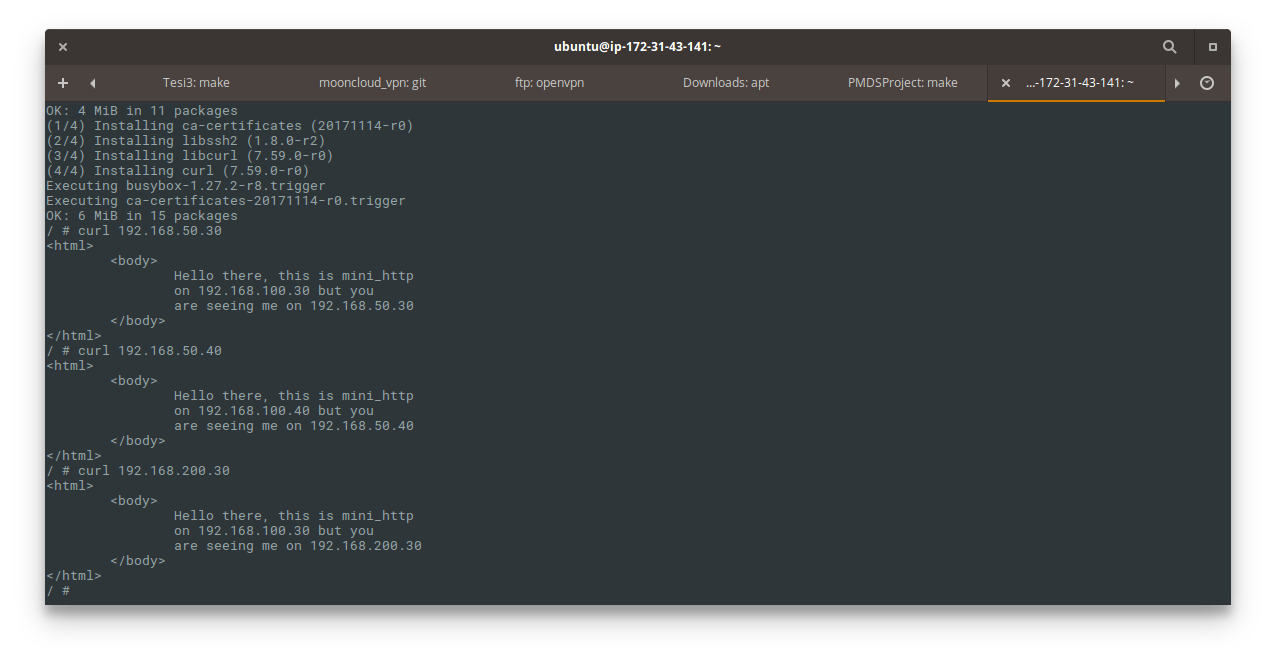
\includegraphics[scale=0.35]{img/test1-result}
  \caption{Il risultato dell'esecuzione del test}
  \label{fig:test1-result}
\end{figure}
A titolo di documetazione, si mostra anche l'output del comando curl eseguito
sui tre host target.
\begin{figure}
  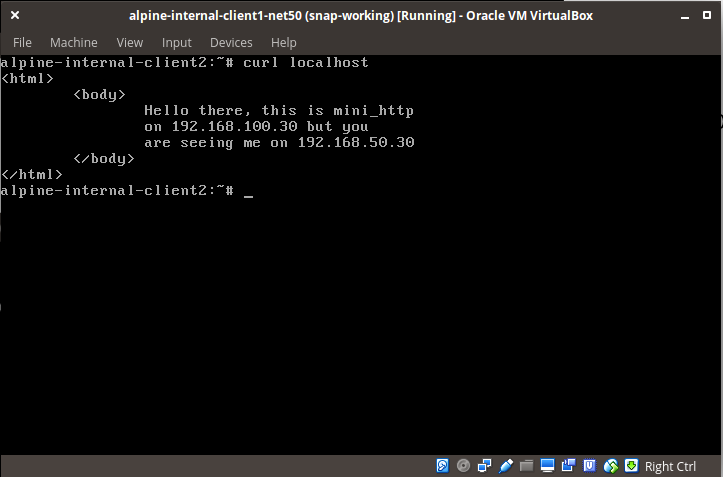
\includegraphics[scale=0.4]{img/alpine-internal-client1-net50}
  \caption[Output di curl su target 1 in \texttt{net50}]
  {L'output di \texttt{curl} su \texttt{192.168.50.30} (mappato)}
  \label{fig:alpine-internal-client1-net50}
\end{figure}
\begin{figure}
  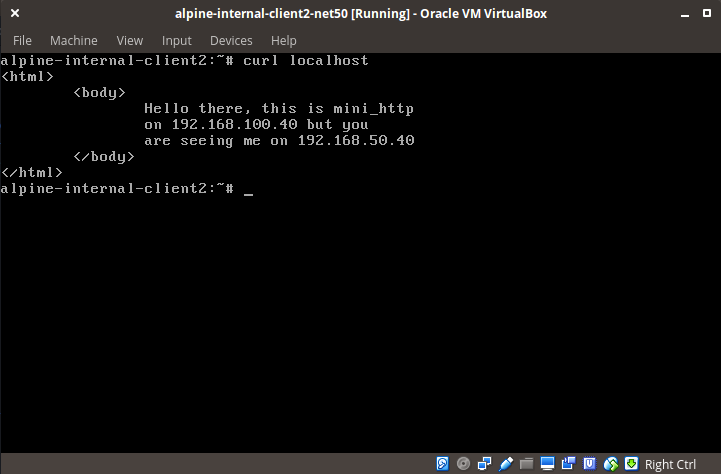
\includegraphics[scale=0.4]{img/alpine-internal-client2-net50}
  \caption[Output di curl su target 2 in \texttt{net50}]
  {L'output di \texttt{curl} su \texttt{192.168.50.40} (mappato)}
  \label{fig:alpine-internal-client2-net50}
\end{figure}
\begin{figure}
  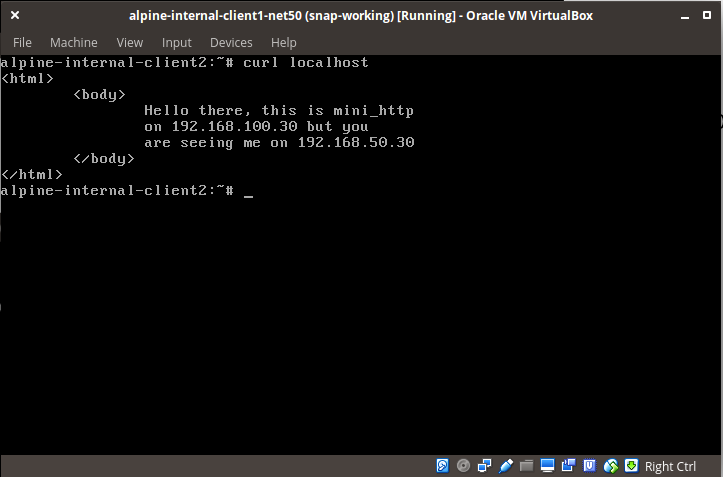
\includegraphics[scale=0.4]{img/alpine-internal-client1-net50}
  \caption[Output di curl su target 3 in \texttt{net200}]
  {L'output di \texttt{curl} su \texttt{192.168.200.30} (mappato)}
  \label{fig:alpine-internal-client-net200}
\end{figure}
